\documentclass[a4paper]{article}
\usepackage[acronym,toc]{glossaries}
\usepackage{url}
\usepackage{graphicx}
\usepackage{float}

\newglossaryentry{bunch}{
   name=bunch,
   description={
      particules trapped inside an \gls{RF} bucket circulating in the 
      machine},
   plural=bunches}
\newglossaryentry{bucket}{
   name={bucket},
   description={
      at every \gls{RF} period in the \gls{rffreq} there is a 
      bucket, in each of these bucket a particles bunch can potentialy be 
      stored in the ring},
   plural={buckets}}
\newglossaryentry{rffreq}{
   name={RF frequency ($f_0$)},
   description={
      the base frequency of the \gls{RF} in the \glspl{cavity} in the case of
      the LHC this frequency is 400.789MHz, this frequency dictate the number of
      bucket that the machine can have}}
\newglossaryentry{cavity}{
   name={cavity},
   description={
      \gls{RF} structure made to accelerate the particles, it uses a high power 
      radio frequency into a resonating structure to increase the energy 
      of the particles},
   plural={cavities}}
\newglossaryentry{VME}{
   name={VMEbus},
   description={
      a computer bus standard widespread at CERN, in the case of the LHC
      \gls{RF} the bus has a larger board and some of the pins are used to 
      route custom signals between cards}}
\newglossaryentry{kicker}{
   name={kicker},
   description={
      machine in an accelerator that can kick the beam transversally, used to
      kick the beam in or out (injection or extraction kicker) of the beam pipe 
      but also in our case excite the beam transversally},
   plural={kickers}}
\newglossaryentry{damper}{
   name={damper},
   description={
      machine in an accelerator that damp the transverse oscilliation of the 
      beam by applying a transverse electric field},
   plural={dampers}}
\newglossaryentry{tune}{
   name={betatron tune},
   description={
      the betatron tune is the frequency of the oscillations of the 
      \glspl{bunch} divided by the \gls{rffreq}}}
\newglossaryentry{h}{
   name={harmonic number ($H$)},
   description={
      the harmonic number is the number of bucket an accelerator can have in 
      the ring, in the case of the \gls{LHC} 35'640}}
\newglossaryentry{FFTW}{
   name={FFTW},
   description={
      is a C subroutine library for computing the discrete Fourier transform 
      (DFT) in one or more dimensions, of arbitrary input size, and of both 
      real and complex data (as well as of even/odd data, i.e. the discrete 
      cosine/sine transforms or DCT/DST)}}

\newacronym{ADT}{ADT}{Accelerating \Gls{damper} Transverse}
\newacronym{MKQA}{MKQA}{tune \gls{kicker}}
\newacronym{BBQ}{BBQ}{diode-based base-band-tune}
\newacronym{LHC}{LHC}{Large Hadron Collider}
\newacronym{DSP}{DSP}{Digital Signal Processor}
\newacronym{FPGA}{FPGA}{Field-Programmable Gate Array}
\newacronym{FFT}{FFT}{Fast Fourier Transform}
\newacronym{GPU}{GPU}{Graphic Processing Unit}
\newacronym{CPU}{CPU}{Central Processing Unit}
\newacronym{BPM}{BPM}{Beam Position Monitor}
\newacronym{RF}{RF}{Radio Frequency}
\newacronym{BI}{BI}{Beam Instrumentation}
\newacronym{CO}{CO}{Control}
\newacronym{OP}{OP}{Operation}
\newacronym{CERN}{CERN}{European organization for nuclear research}
\newacronym{MD}{MD}{Machine Developpment}

\makeglossaries

\title{Betatron tune measurement in the LHC using GPU}
\author{Fr\'ed\'eric Dubouchet}
\date{\today}

\begin{document}

\maketitle
\tableofcontents

\begin{abstract}
This paper describes the betatron tune measurement in the \gls{LHC} at the
\gls{CERN} including the present hardware and the future possible 
implementations using the \gls{ADT} acquisitions. The \gls{ADT} data have to 
be processed to be able to extract the \gls{tune}. This paper studies the use
of \glspl{GPU} to process \gls{bunch} position acquisition data.
\end{abstract}

\clearpage

\section{Introduction}

In a particle accelerator, the charged particles circulate around the ring
and oscillate due to the magnets and the accelerating structures. The 
accelerating structures, in the \gls{LHC} supra-conducting \glspl{cavity} 
apply a strong electrical field that oscillates at the \gls{rffreq} 
to particles in order to collect and accelerate particles in \glspl{bunch} 
inside a frequency \gls{bucket}.

The particles inside a bucket are oscillating longitudinally along the 
ring and transversally in the vertical and horizontal plane. The longitudinal
oscillations are damped by the beam control system. But the transversal
oscillations must be damped by a separate system~: the 
\gls{ADT}\cite{Benews11,Zhabitsky:1141925}.

One of the key parameters of the accelerator is the betatron tune. The 
betatron tune, $Q$, is the quotient of the betatron oscillation and the 
particle frequencies.

$$f_\beta = Q * f_0$$

This value allow us to check if the particle beam is stable and don't reach
any dangerous instabilities.

\section{Tune measurement in the LHC}

In order to measure the betatron tune in an accelerator we use \glspl{BPM}.
These monitors are able to measure the position of the beam in the vacuum 
chamber.

\subsection{Actual system}

In the present setup \gls{BI} group is using their \gls{BBQ} 
\cite{Boccardi:1156349} system to acquire the tune over a certain number
of machine turn (256 to 128'000). This can work as a passive instrument or as 
an on demand system by exciting 12 \glspl{bunch} in the beam with the 
\gls{MKQA}. \Gls{ADT} has also been used for tune measurement 
excitation\cite{HofleEvian10}. 

In normal operation, as the \gls{ADT} is active, it is difficult to have a
good picture of the excited bunches and make a fine tune measurement~: the
oscillations created by the \gls{MKQA} are damped by the \gls{ADT}. There
have been studies to disable the \gls{ADT} for a certain number of bunches in
order to get a better tune measurement\cite{HofleEvian11}, but this may
not be sufficient.

\subsection{Proposed system}

The \gls{ADT} also have \glspl{BPM} and these can have per bunch 
measurement\cite{BphMeas07}. This could allow a much precise measurement. But due 
to the high among of data to be processed (estimated to 640 mega bytes per 
seconds for each \gls{BPM}) we need dedicated hardware to compute the 
correct tune\cite{HofleChamonix12}.

During the 2012 normal operation of the \gls{LHC}, data will be acquired using
the \gls{ADT} acquisition system and data processing techniques will be 
tried to asses the modification that will be needed in order to make a 
reliable \gls{tune} measurement at a reasonable rate\cite{HofleChamonix12}.

The current \gls{VME} implementation has some serious issues in particular 
the bus is quite slow the data rate of the bus is around 40 megabits per 
seconds. The data need to either be processed on the acquisition board or 
to be off-loaded to another computer using the serial link available on the 
board\cite{Baudrenghien:1124094}.

\subsubsection{DSP on VME board}

\Glspl{DSP} are able to compute \glspl{FFT} at high rate and these are used
already in the machine at different places to make high speed feedback loops.
The question is~: is it fast enough to compute all the \glspl{FFT} needed, 
\glspl{DSP} are two orders of magnitude slower than \glspl{GPU}. We also 
would have to develop a completely new system in order to be able to use them, 
in fact we don't have \glspl{DSP} in the present \gls{ADT}. The cost of 
development and the complexity of the deployment should also be studied.

\subsubsection{FPGA pre-processing on VME board}

Like in the approach using \glspl{DSP} on VME boards, the question of computing 
power is still unsolved. We already have in house experience and we already 
have a lot of \gls{FPGA} installed in the \gls{ADT}. But if we want to do it we 
will have to create a new card able to replace the existing one and to make the 
computation. This mean create a potential problem in the existing setup. The 
cost is also to be studied we have to develop a new card, test it and install 
it in the \gls{LHC}.

\subsubsection{GPU off-board computing}

This solution can be integrated easily in the present setup. The present 
acquisition cards already have a digital output and could be used to transfer
the data in another crate that could do the computations. The \glspl{GPU} are
cheap (compare to the price of developing a new \gls{VME} card) and easily
scalable. The \gls{GPU} should have largely enough computing power to be able
to make the \glspl{FFT}. Another interesting aspect of this solution is the 
ability to test it using \gls{CPU}.

\section{Estimation of the amount of data}

Presently the \gls{LHC} is working with an interval of 50ns between 
\glspl{bunch} this correspond to a bunch every 10 \glspl{bucket}. But the 
\gls{OP} is planning to move to 25ns \glspl{bunch} spacing this would mean 
5 \glspl{bucket} between \glspl{bunch}. With the \gls{rffreq} we can compute 
the number of acquisitions per seconds.

$$for~50~ns~: \frac{400.789M}{20} = 20'039'450 \leq 2^{25}$$

$$for~25~ns~: \frac{400.789M}{10} = 40'078'900 \leq 2^{26}$$ 

This represent the amount of data for one pickup (\gls{BPM}), in the case of 
\gls{ADT} we have two of them per beam and per plane so as the \gls{LHC} has 
two rings and for each ring there are two transversal plane and there are 
two pickups per plane. This means we still have to multiply this value by 
eight.

$$for~50~ns~: 2^{25} * 8 = 2^{28}$$

$$for~25~ns~: 2^{26} * 8 = 2^{29}$$

As \glspl{FFT} on \glspl{GPU} start to be be faster than \glspl{CPU} around 
$2^{15}$ acquisitions it seems interesting to study this kind of system to 
compute the \gls{tune}.

\section{Measurement with the ADT}

\begin{figure}[H]
\caption{Spectrogram of the beam position taken on the 16 October 2012}
\centering
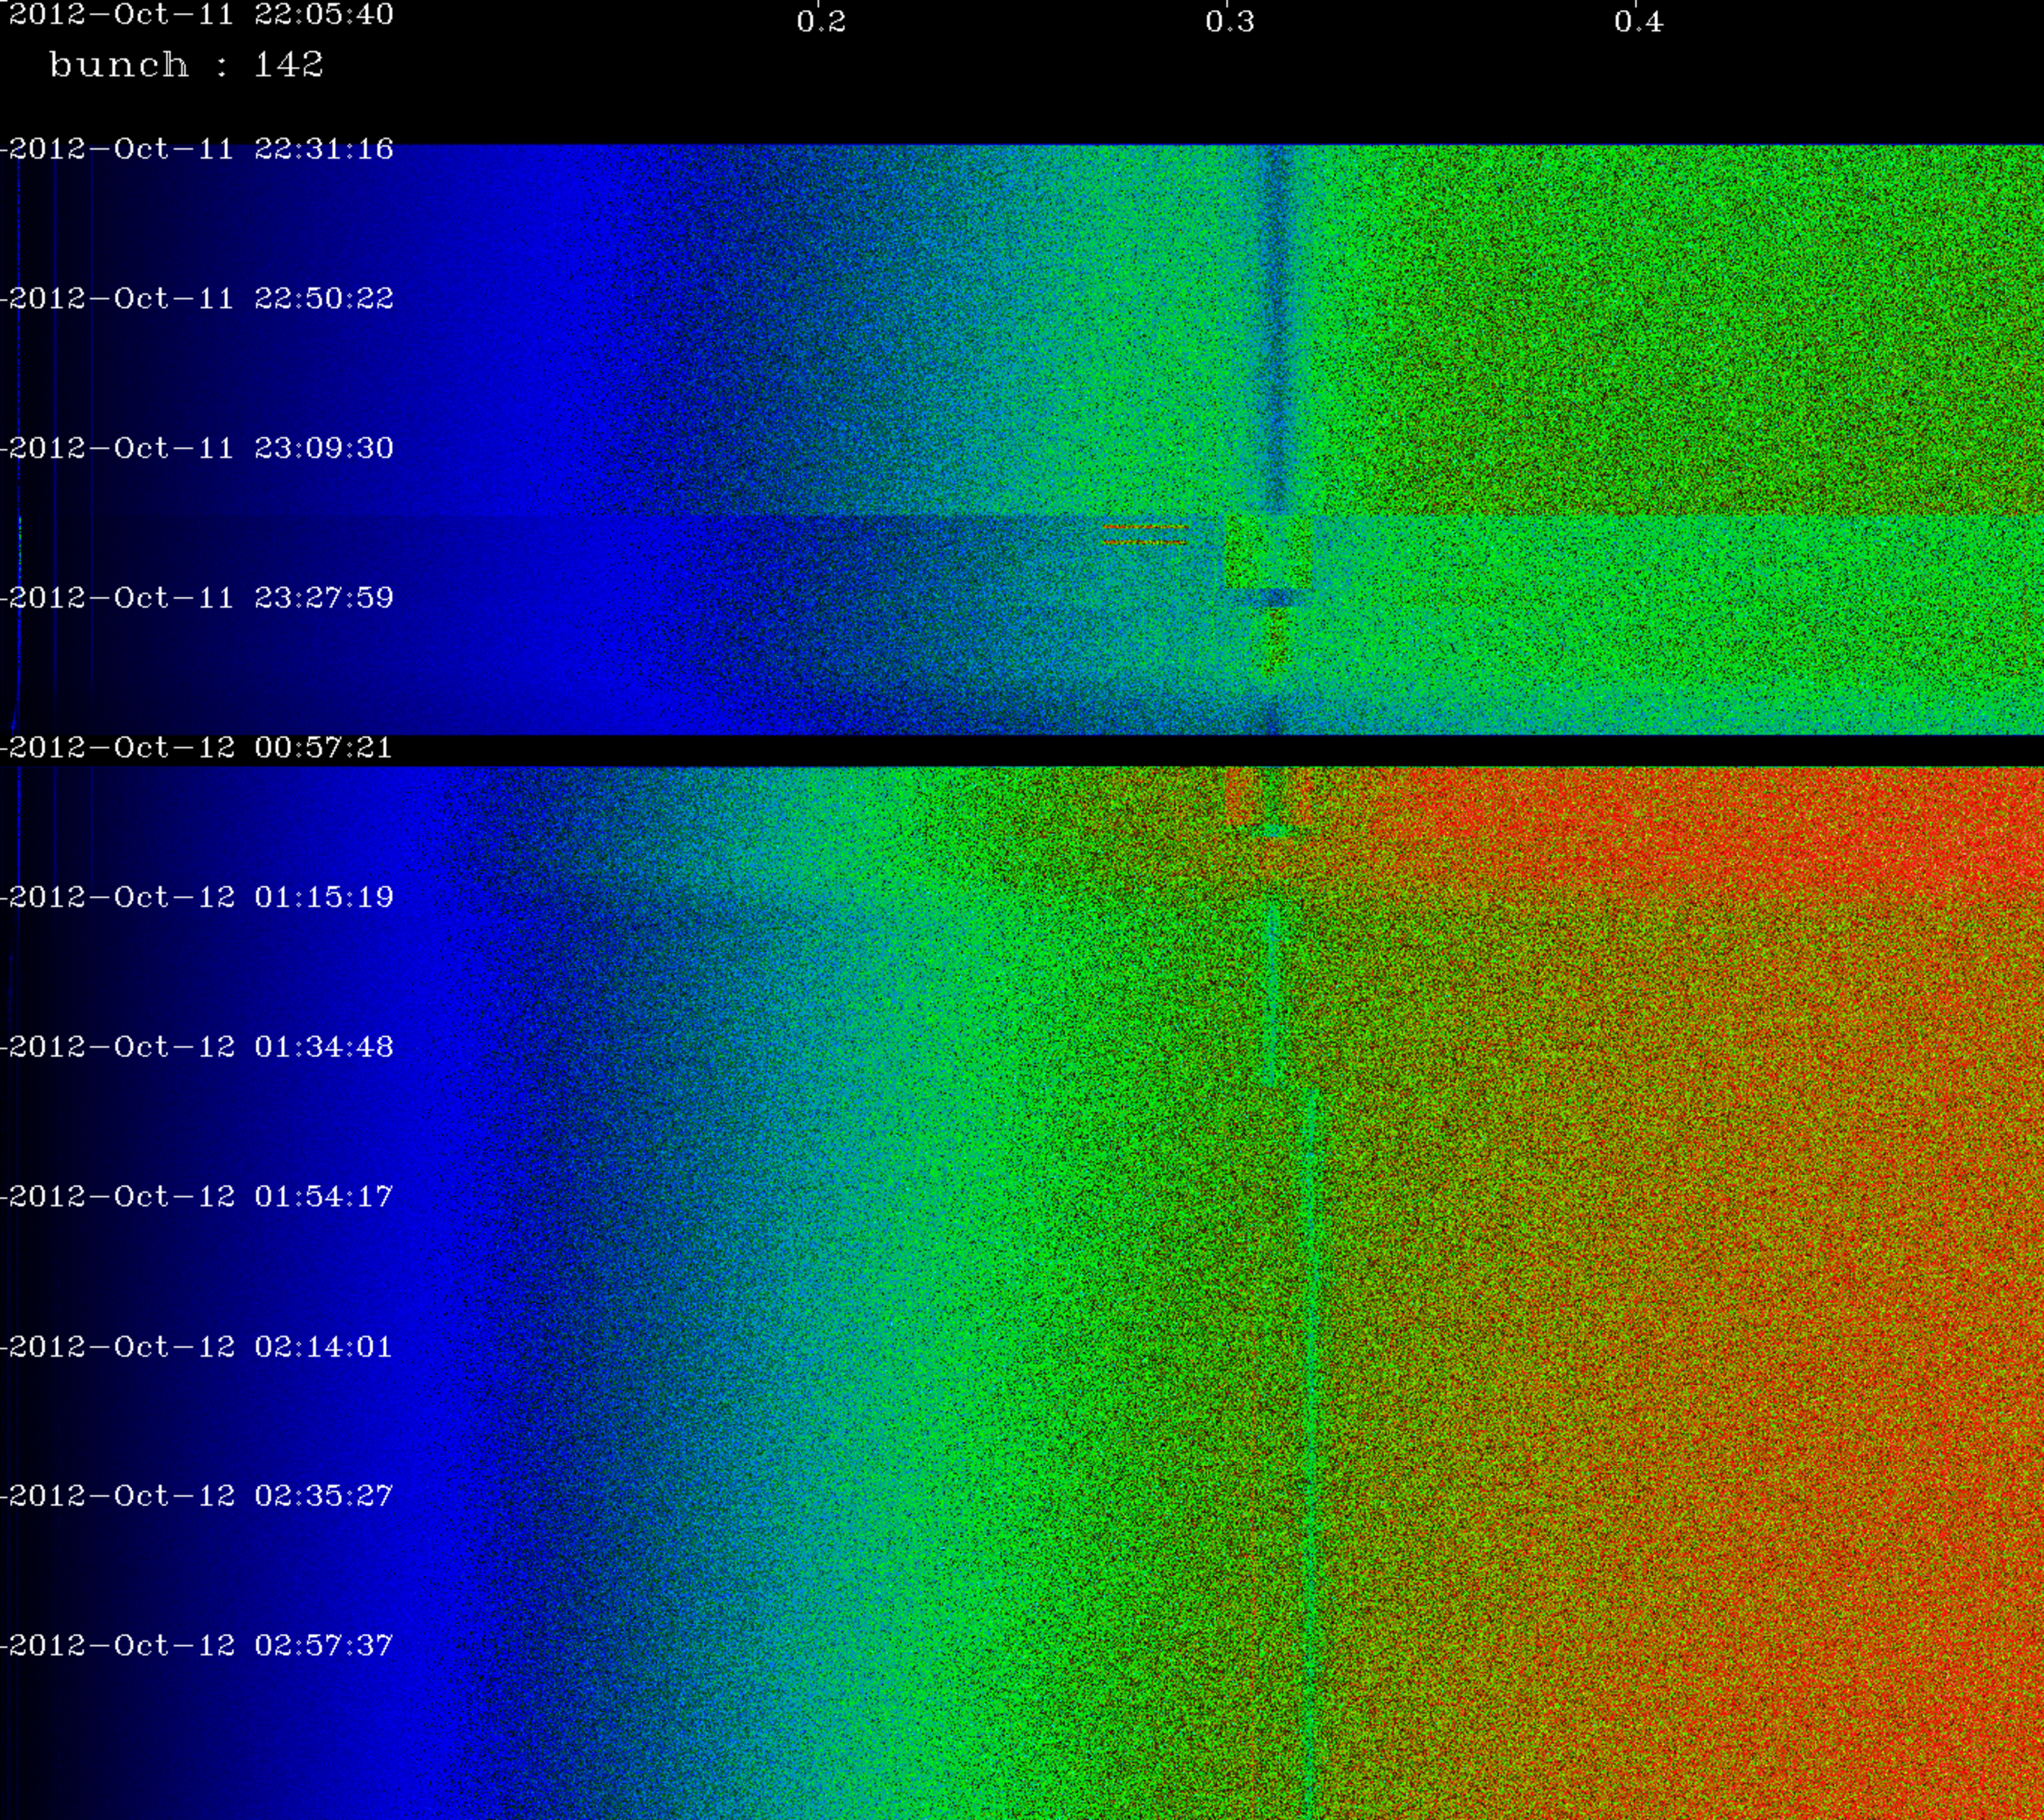
\includegraphics[scale=0.2]{spectrogram.pdf}
\end{figure}

In order to check the feasibility of the system and to have a good prototype
the first test will be to excite some of the \glspl{bunch} and acquire the
\gls{tune} using the \gls{ADT} during the end of 2012 run.

A piece of software has been developed that will acquire the bunch by bunch 
acquisition and compute various algorithm on the data using the \gls{CPU} 
and the \gls{FFTW} library in the \gls{CERN} infrastructure using \gls{CO} 
group control system and the \gls{OP} group infrastructure.

\section{Proposed implementation}

\begin{figure}[H]
\caption{ADT acquisition hardware}
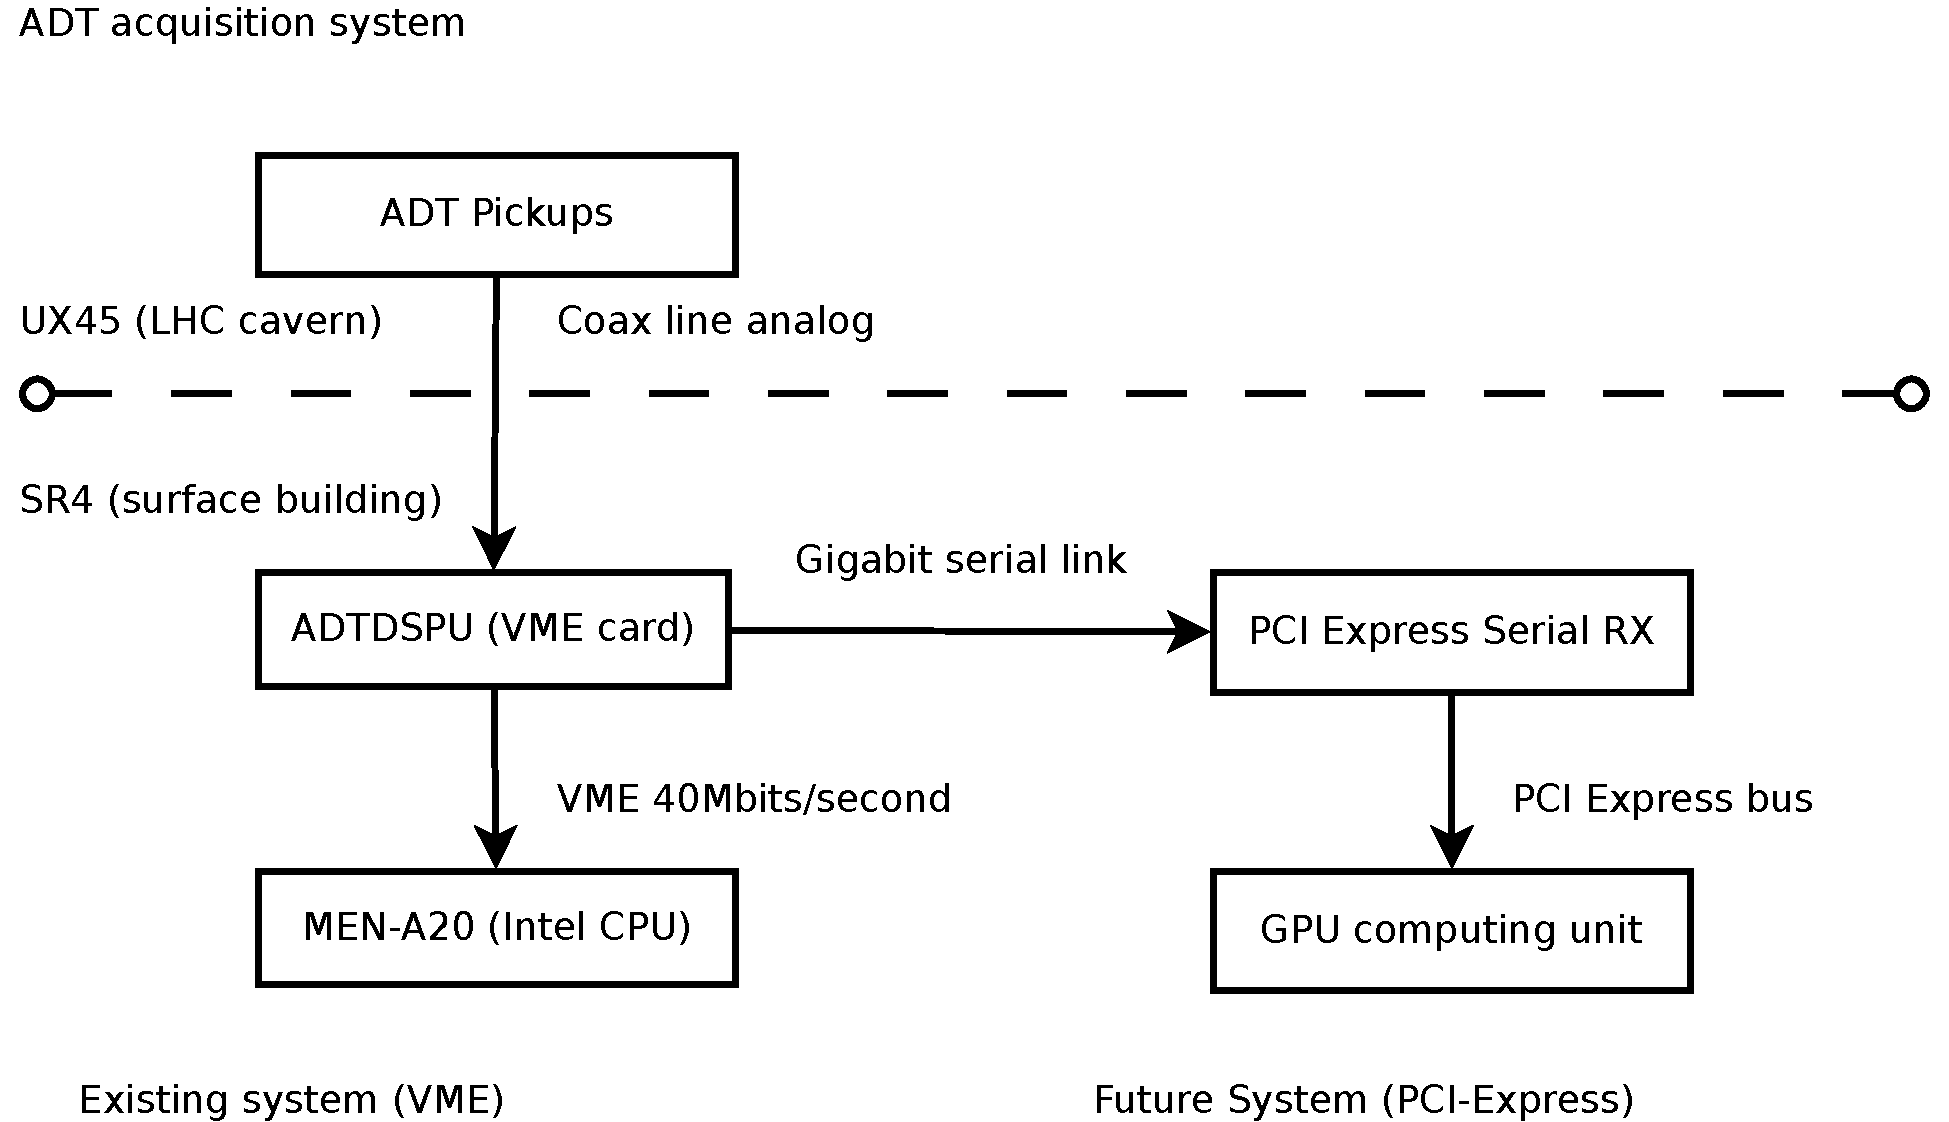
\includegraphics[scale=0.3]{acquisition.pdf}
\end{figure}

\begin{figure}[H]
\caption{Acquisition data flow}
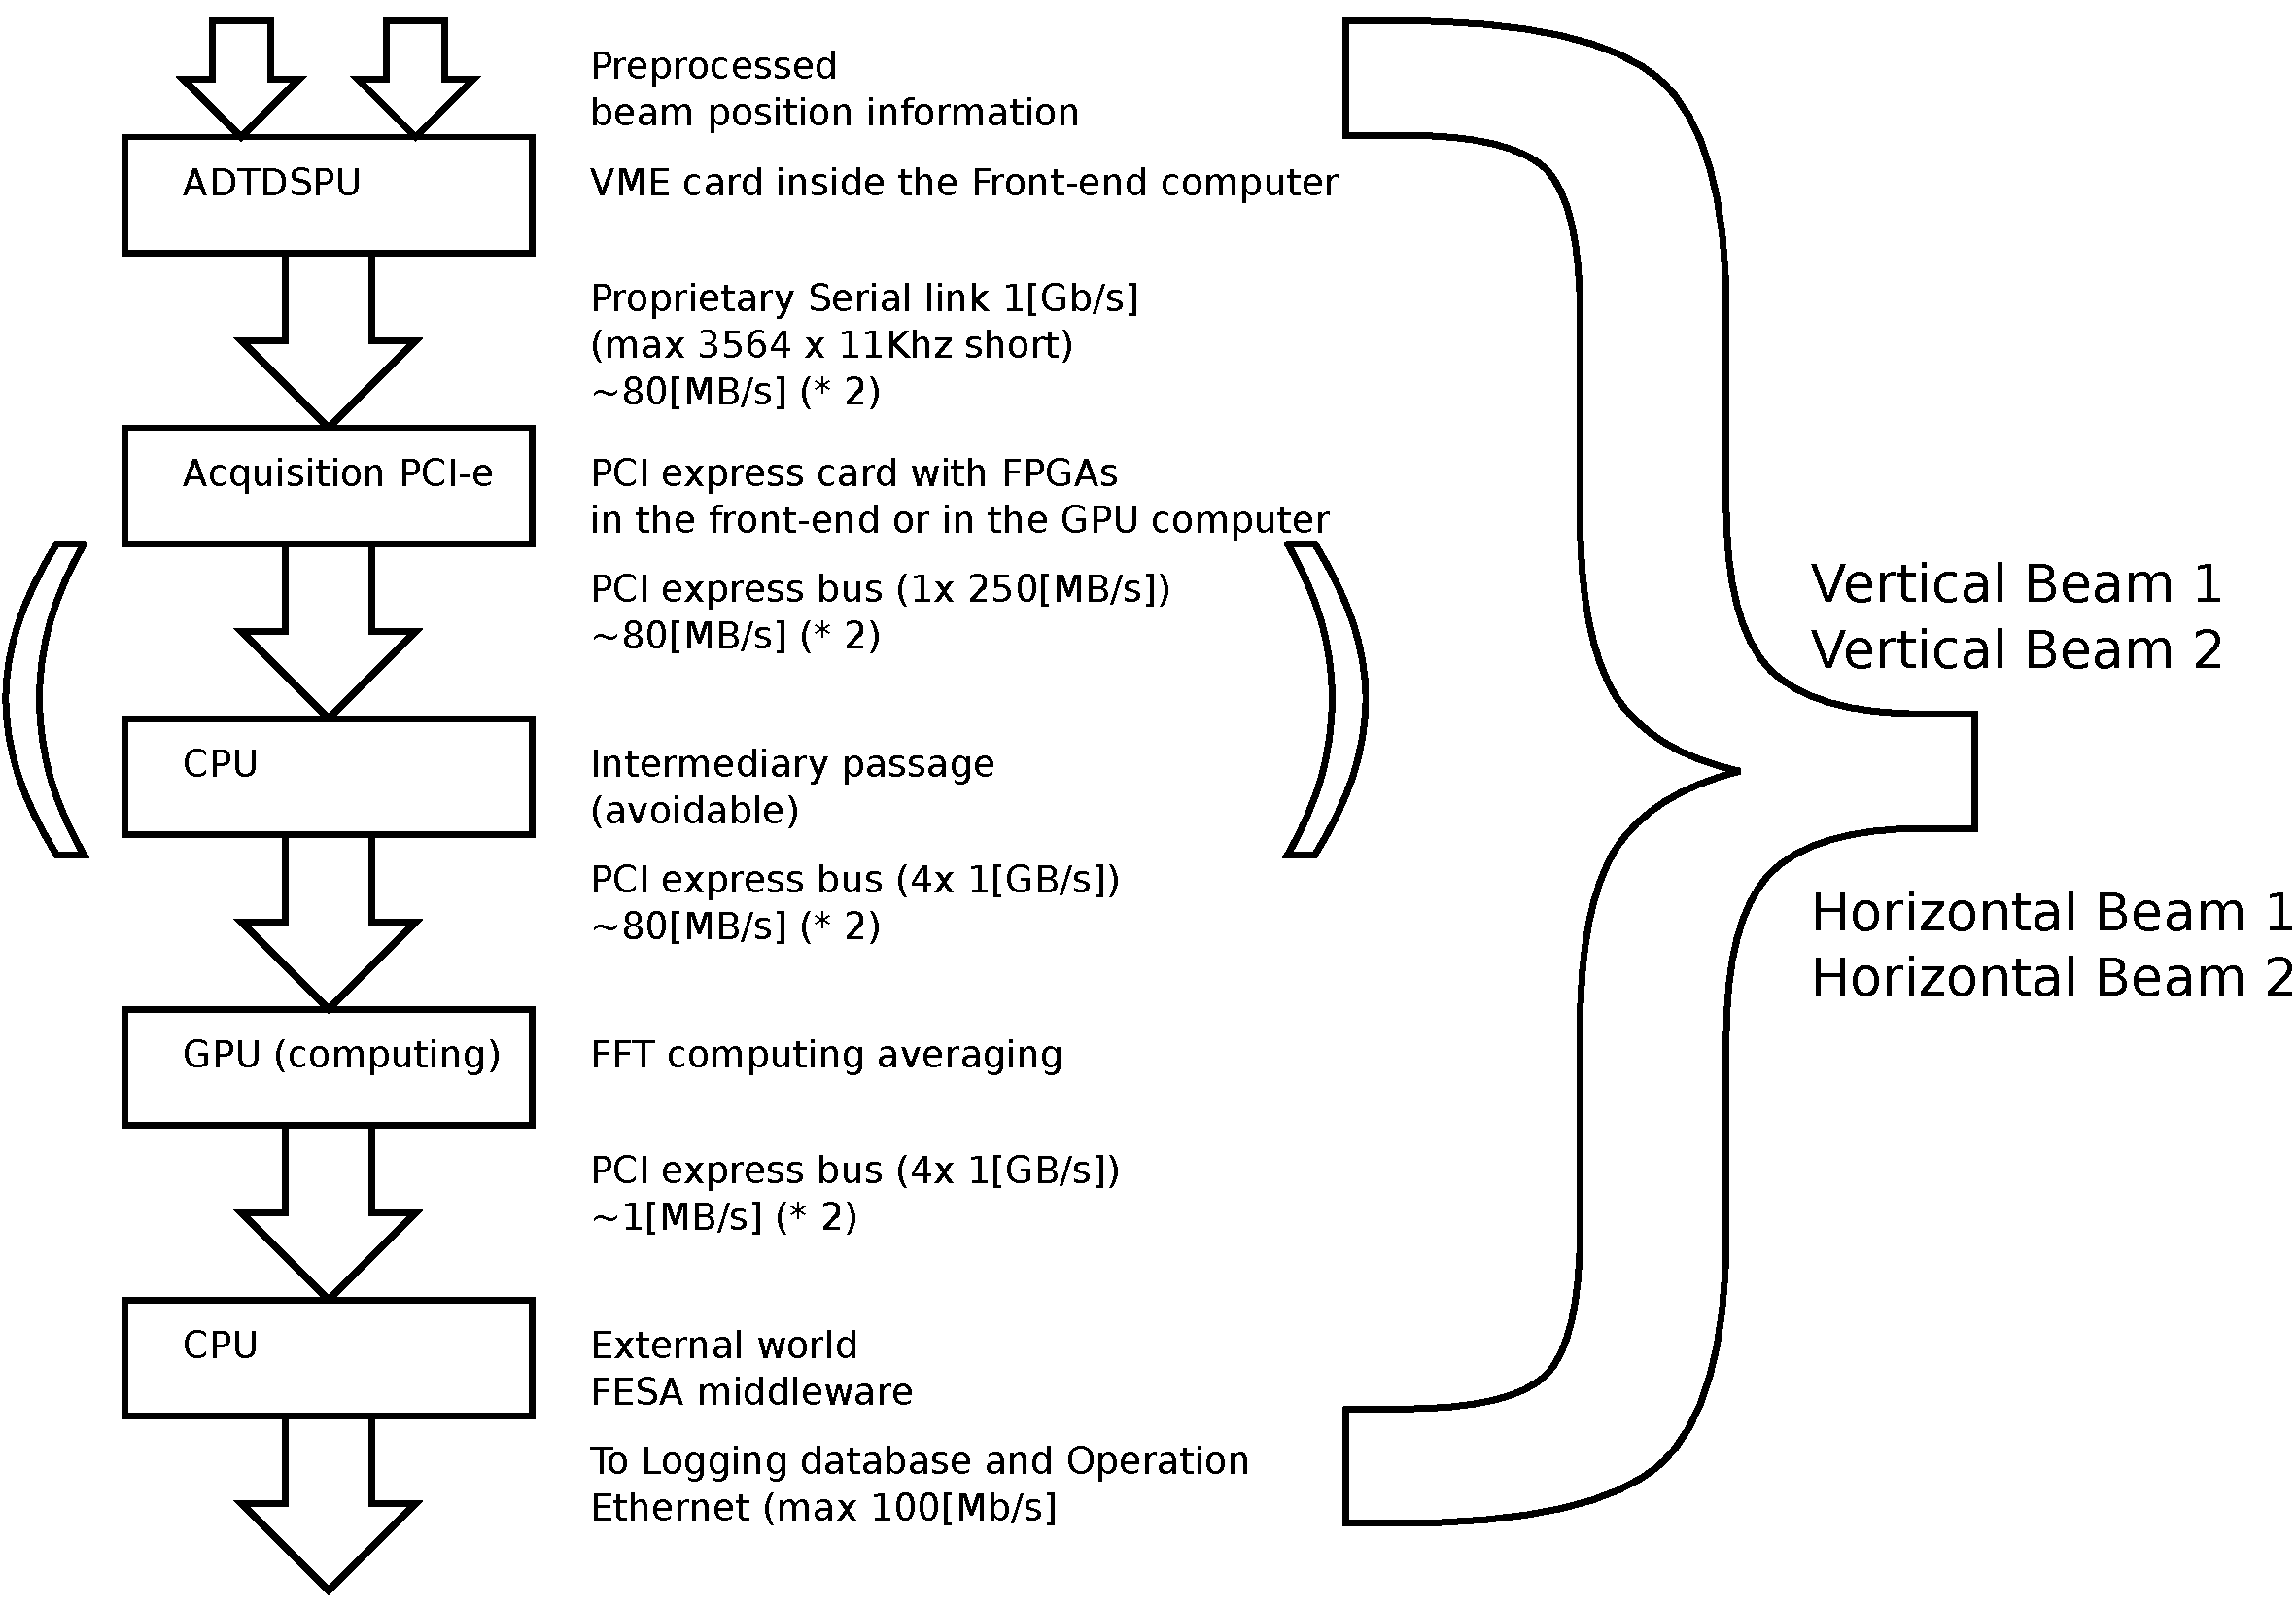
\includegraphics[scale=0.3]{dataflow.pdf}
\end{figure}

\section{Conclusion}

This project looks like a nice place to try using \glspl{GPU} in accelerators.
The possibilities are promising and the gain for the stability of the 
\gls{LHC} could allow more physic time. \Glspl{GPU} could prove to be useful
and be used in other places in accelerators where computing power is needed.

\printglossaries

\clearpage

\bibliographystyle{plain}
\bibliography{bibliography}

\end{document}

